\documentclass[12pt]{article}
\usepackage{amsmath}
\usepackage{amssymb}
\usepackage{geometry}
\usepackage{enumerate}
\usepackage{natbib}
\usepackage{float}%稳定图片位置
\usepackage{graphicx}%画图
\usepackage[english]{babel}
\usepackage{a4wide}
\usepackage{indentfirst}%缩进
\usepackage{enumerate}%加序号
\usepackage{multirow}%合并行


\begin{document}
\newpage
\section{Problem 1}
\subsection{(a)}
$$I_c=I_s \exp(\frac{q V_{BE}}{KT}-1)(1+\frac{V_{CE}}{V_A})=10^{-16}\exp(\frac{0.7}{0.0259}-1)(1+\frac{V_{CE}}{100})=5.47\cdot10^{-5}*(1+0.01*V_{OUT})$$
$$V_{OUT}=V_{CC}-R_c*I_c=3-5000I_c$$
$$V_{OUT}=2.72(V)$$
$$I_c=\frac{3-2.9}{5000}=5.6\cdot10^{-5}(A)$$
$$gm=\frac{q\cdot I_c}{KT}=\frac{5.6\cdot10^{-5}}{0.0259}=2.162\cdot10^{-3}$$
$$r_0=\frac{V_A}{I_c}=\frac{100}{2.07\cdot 10^{-5}}=1.79\cdot10^{6}(\Omega)$$
$$A_v=-gm(R_c||r_0)=-2.162\cdot10^{-3}\cdot\frac{5000*1.79\cdot10^{6}}{5000+1.79\cdot10^{6}}=-10.78$$
\subsection{(b)}
\begin{figure}[H]
\centering
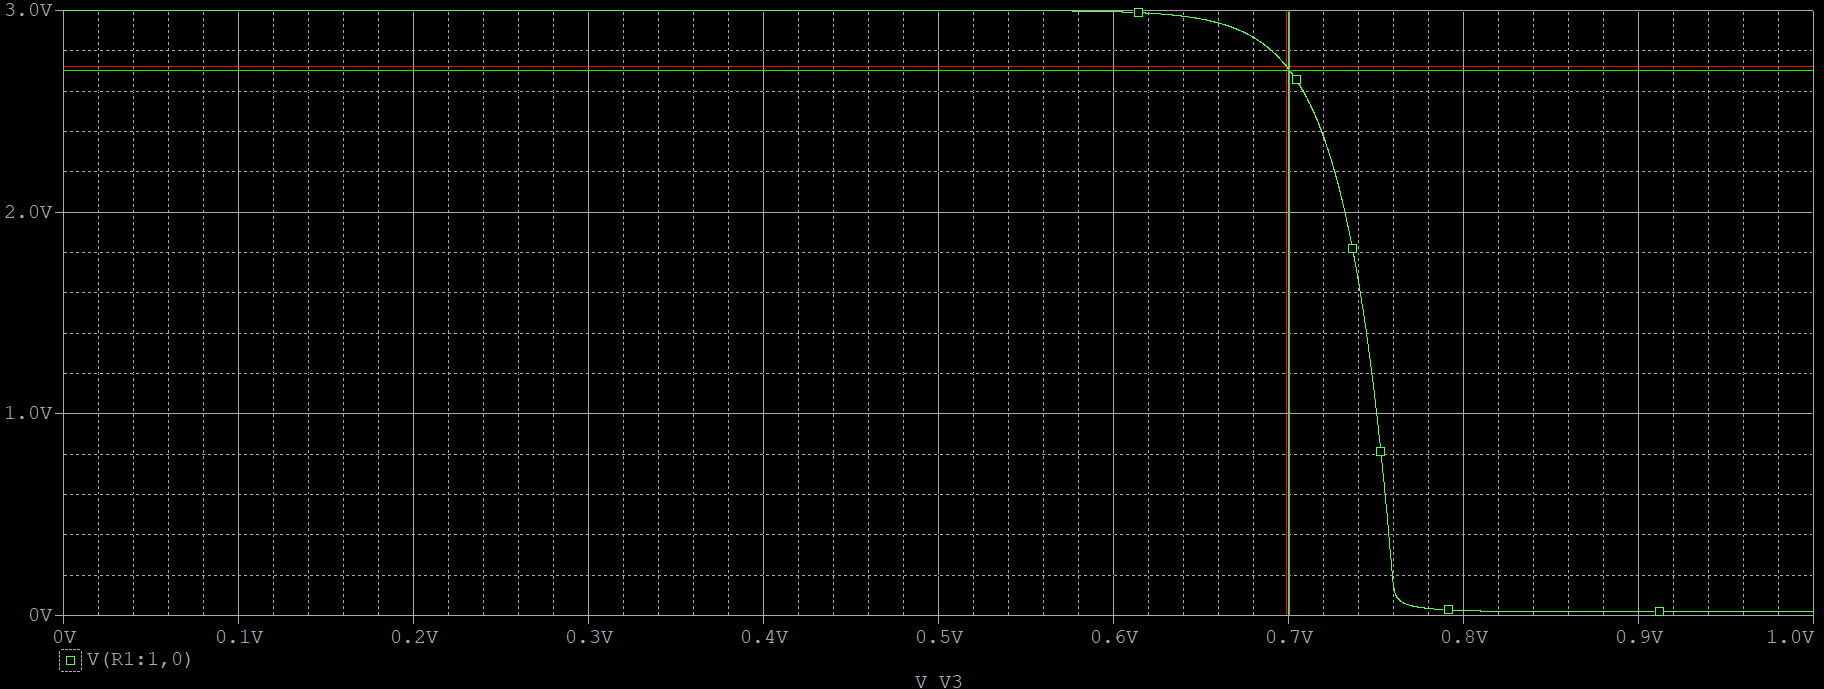
\includegraphics[scale=0.25]{P1.png}
\end{figure}
$$A_v=\frac{18}{-1.7}=-10.6$$
The slope is about -10.6, which is a little bigger than calculated one in (a)
\subsection{(c)}
\begin{figure}[H]
\centering
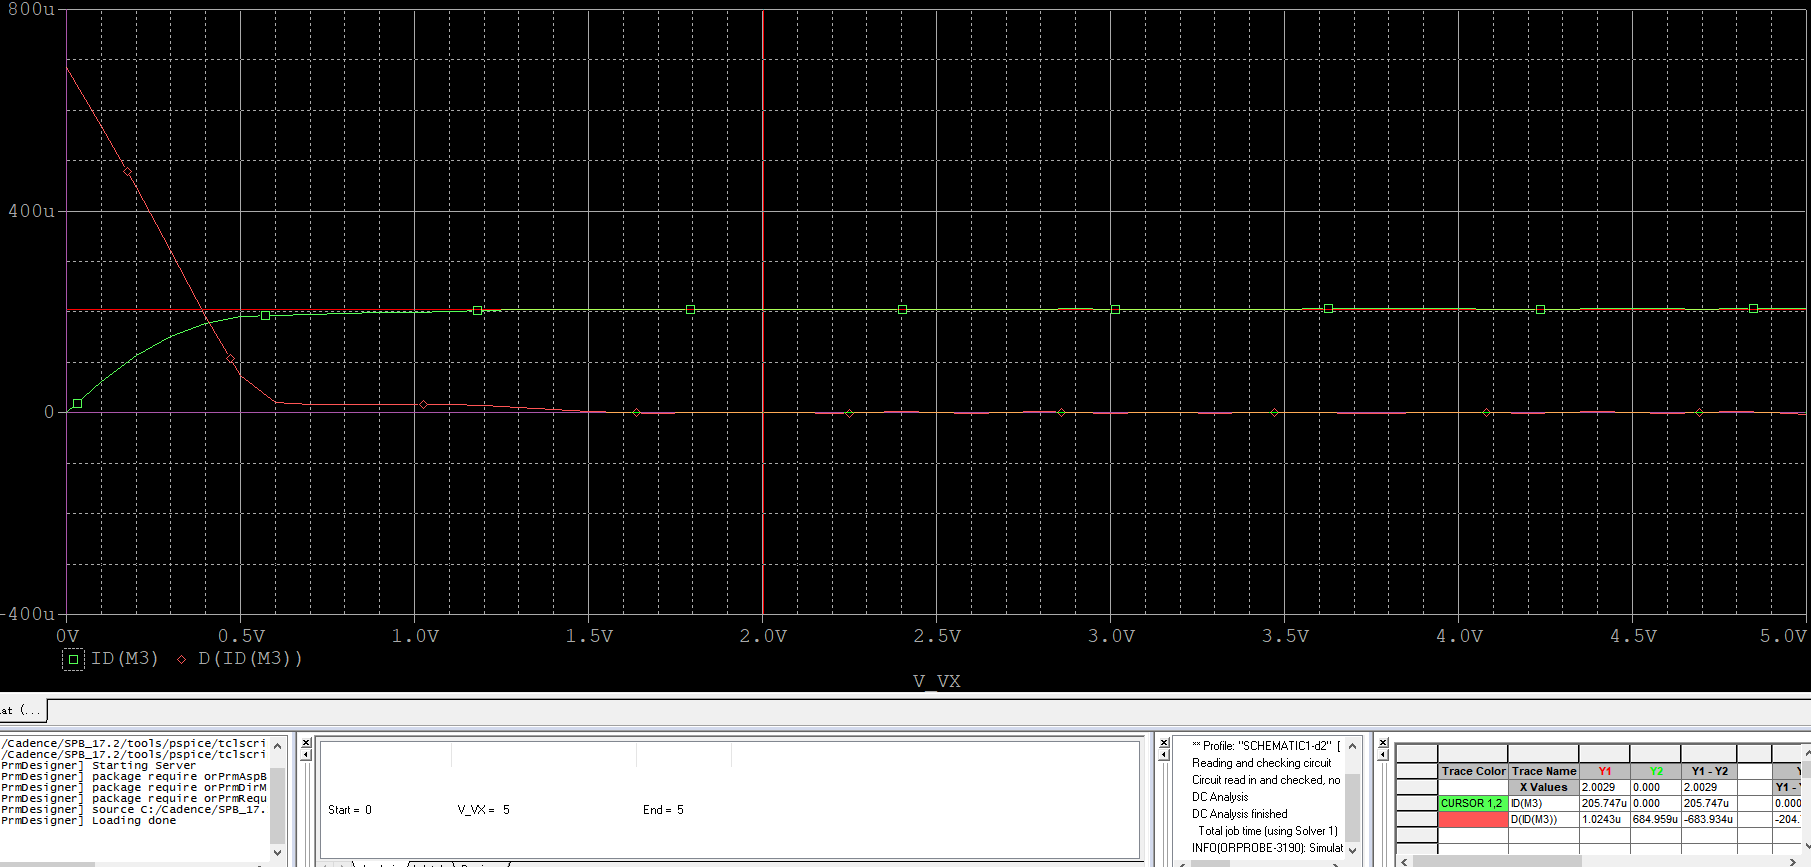
\includegraphics[scale=0.25]{P2.png}
\end{figure}
$$|A_v|=|\frac{(2.8-2.9)}{0.69-0.7}|\approx10$$
The value is very close to part (b) and (a) but the absolute value is a bit smaller.
\subsection{(d)}
\begin{figure}[H]
\centering
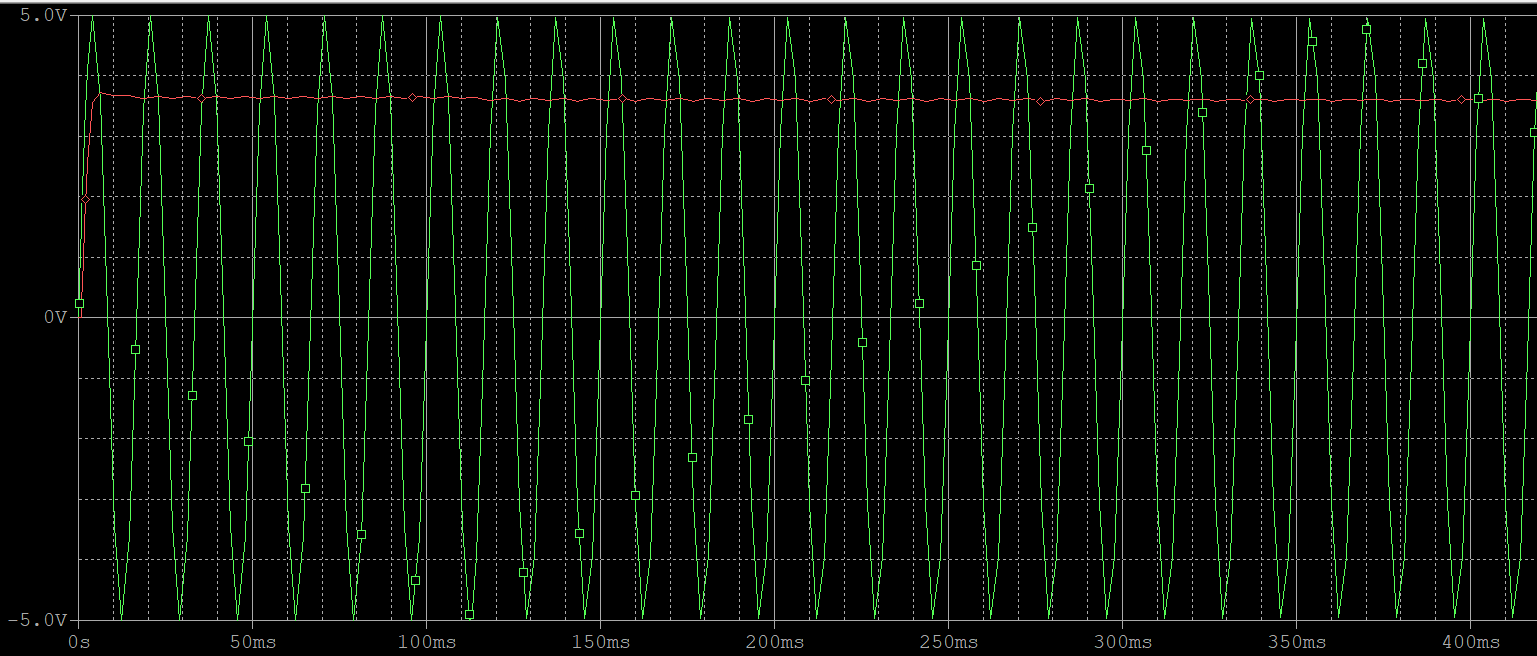
\includegraphics[scale=0.25]{P3.png}
\end{figure}
$$|A_v|=|\frac{(2.96-2.9)}{0.65-0.7}|\approx47.2$$
The value is much more greater than calculated one in previous part, I think it's because the amplitude is so big that the input signal can't be considered as a small signal any more. As a result, the derivative for $V_{BE}$ can't be applied any more gm has changed.
\end{document}